\title{WED2 CheatSheet}
\author{dthoma & lroellin}
\date{Juli 2018}

\documentclass[a4paper, fontsize=6pt]{scrartcl}
\usepackage{multicol}
\usepackage{calc}
\usepackage{ifthen}
\usepackage[landscape]{geometry}
\usepackage{hyperref}
\usepackage{graphicx}
\usepackage{mathtools}
\usepackage{gensymb}
\usepackage{minted}
\setminted{fontsize=\footnotesize,baselinestretch=1}
\usemintedstyle{vs}
\usepackage{ragged2e} 
\usepackage[T1]{fontenc}
\usepackage[utf8]{inputenc}
\usepackage[shorthands=off,ngerman]{babel}
\usepackage{amsbsy}
\usepackage{amsfonts}
\usepackage{varwidth,pst-tree,pst-eps}
\usepackage{comment}
\usepackage{xcolor}
\usepackage{titlesec}
\usepackage{tikz}
\usetikzlibrary{shapes,arrows}

\usepackage{fontspec}

\setromanfont[
Path=fonts/Roboto/,
BoldFont=Roboto-Bold.ttf,
ItalicFont=Roboto-Italic.ttf,
BoldItalicFont=Roboto-BoldItalic.ttf
]{Roboto-Regular.ttf}
\setmonofont[
Path=fonts/Hack/,
BoldFont=Hack-Bold.ttf,
ItalicFont=Hack-Italic.ttf,
BoldItalicFont=Hack-BoldItalic.ttf
]{Hack-Regular.ttf}

\AtBeginEnvironment{minted}{%
  \renewcommand{\fcolorbox}[4][]{#4}}

%German-specific commands
%--------------------------------------
% \usepackage[german]{babel} % wegen "s => ß disabled
%--------------------------------------

\graphicspath{ {images/} }


% This sets page margins to .5 inch if using letter paper, and to 1cm
% if using A4 paper. (This probably isn't strictly necessary.)
% If using another size paper, use default 1cm margins.
\geometry{top=0.5cm,left=0.5cm,right=0.5cm,bottom=0.5cm}

% Turn off header and footer
\pagestyle{empty}
 

% Redefine section commands to use less space
\makeatletter
\renewcommand{\section}{\@startsection{section}{1}{0mm}%
    {-1ex plus -.5ex minus -.2ex}%
    {0.5ex plus .2ex}%x
    {\normalfont\large\bfseries}}
    
\renewcommand{\subsection}{\@startsection{subsection}{2}{0mm}%
    {-1explus -.5ex minus -.2ex}%
    {0.5ex plus .2ex}%
    {\normalfont\normalsize\bfseries}}
    
\renewcommand{\subsubsection}{\@startsection{subsubsection}{3}{0mm}%
    {-1ex plus -.5ex minus -.2ex}%
    {1ex plus .2ex}%
    {\normalfont\small\bfseries}}
    
\makeatother

% Define BibTeX command
\def\BibTeX{{\rm B\kern-.05em{\sc i\kern-.025em b}\kern-.08em
    T\kern-.1667em\lower.7ex\hbox{E}\kern-.125emX}}

% Don't print section numbers
%\setcounter{secnumdepth}{0}


\setlength{\parindent}{0pt}
\setlength{\parskip}{0pt plus 0.1em}

\titlespacing{\paragraph}{%
  0pt}{%              left margin
  0.5\baselineskip}{% space before (vertical)
  1em}%               space after (horizontal)

\newcommand{\css}[1]{\texttt{#1}}
\newcommand{\scss}[1]{\mintinline{scss}{#1}} % mit minted, wegen den Steuerzeichen
\newcommand{\html}[1]{\texttt{#1}}
\newcommand{\js}[1]{\texttt{#1}}


% -----------------------------------------------------------------------

\begin{document}

\footnotesize
\begin{multicols*}{5}


% multicol parameters
% These lengths are set only within the two main columns
%\setlength{\columnseprule}{0.25pt}
\setlength{\premulticols}{1pt}
\setlength{\postmulticols}{1pt}
\setlength{\multicolsep}{1pt}
\setlength{\columnsep}{2pt}

Partnerarbeit von lroellin und dthoma

\section{REST}
% Eigenschaften von Rest (04 12 & 17) LOW PRIO

% ROA Prinzipien erwähnen (04 20) LOW PRIO
% Resource Links erwähnen (04 22)
\textbf{URL Regeln}
Ressourcen werden immer mit einer URL identifiziert (Resource Oriented Architecture \textbf{ROA}). Ressourcen in Mehrzahl, Query-Parameter nur für Algorithmen oder Filter (\texttt{/orders?state=delay}). Hat man verlinkte Ressourcen, so kann man sie entweder direkt in der Antwort mitgeben, oder die URL zum Abruf dieser Ressource zurückgeben.

% HTTP-Verben und ihre Semantik KURZ aufschlüsseln (04 23ff)
\textbf{HTTP-Methoden} 
\textbf{GET}: abrufen, Accept-Header definiert Repräsentation. Status-Codes beachten. \textbf{POST}: neue Ressource erzeugen. \texttt{Content-Type} Header angeben. Wenn die Ressource erzeugt wird, im Response-Header. \texttt{Location} die URI angeben. Kein Cache. \textbf{PUT} aktualisiert eine Ressource, oder erzeugt sie falls noch nicht vorhanden. Idempotent! Kein Cache. \textbf{DELETE} löscht eine Ressource. Kein Cache. \textbf{OPTIONS} gibt an, wie die Ressource verwendet werden darf, z.B. welche Methoden erlaubt sind. \textbf{HEAD} genau gleich wie GET, aber ohne die eigentliche Ressource. Mit Cache. Header-Informationen und Statuscodes sind relevant. \textbf{PATCH} wird für partielles Updaten genutzt.
% Resource Repräsentation erwähnen (04 33) LOW PRIO
\textbf{Repräsentation} 
Wie die Ressource schlussendlich repräsentiert werden soll (JSON, XML, Excel-Tabelle, ...) entscheidet der \texttt{Accept-Request}-Header

% HATEOEAS Prinzip erwähnen ("Browsable API", https://spring.io/understanding/HATEOAS) (04 38)
\textbf{HATEOEAS} 
Hypermedia as the engine of application state. "Browsable API", selbstbeschreibend, technisch sehr schwer umsetzbar.

\textbf{Versionierung}
Oftmals ein Knackpunkt. In der Realität oft über URL, auch wenn das ROA widerspricht. Andere Varianten wären der Media-Type im Accept. Am besten: keine Versionierung

\textbf{Best Practices}
Use nouns but no verbs. Use plural nouns. Use HTTP status codes. Respect the meaning of the HTTP methods: GET method should not alter the state. PUT is idempotent, POST is not idempotent.
\section{Responsive Design}
% TODO: Responsive Design (Media Queries) display, flex-direction, flex-wrap, justify-content, align-items, align-content, order, flex, align-self

% Device Pixel erwähnen (06 23)
\textbf{Device Pixel}
CSS-Pixel sind nicht Device-Pixel. Smartphones haben unterschiedliche Pixel Ratios.

% Prinzipien Graceful Degradation/Progressive Enhancement KURZ erklären (06 26)
\textbf{Browser nicht auf dem selben Stand}
Zwei Vorgehensweisen. \textbf{Graceful Degradation} Alle modernen Features nutzen. Bei älteren Brwosern Polyfills nutzen, sinnvolle Alternative geben oder auf Problem hinweisen. \textbf{Progressive Enhancement} für alle Browser zugänglich machen. Mit Grundfunktionalität starten (kein JS, keine Media Queries), dann mit zusätzlichem CSS und JS Zusatzfunktionalität bieten.

% @support (06 32) LOW PRIO
% modernizr erwähnen (06 33) LOW PRIO
\textbf{Support abfragen}
Mit \css{\@supports (flex-wrap: wrap) \{\}} kann abgefragt werden, ob ein Browser ein Feature unterstützt. Es gibt aber auch den Modernizr.

% Responsive Image Varianten (06 39/40) mittlere PRIO
\textbf{Responsive Images}
\html{src} Fallback, \html{srcset} Liste von Bildern mit zusätzlichen Informationen wie Grösse oder Pixeldichte, \html{sizes} gibt an, wie gross das Bild im Layout sein sollte (\css{[media query] [length], [media query] [length]}). Browser wählt aus!

\begin{minted}{html}
<img src="image-src.png" srcset="300.png 300w, 
  600.png 600w"sizes="(max-width: 320px) 49vw, 100vw">
<img src="image-src.png"  srcset="image-1x.png 1x,
  image-2x.png 2x, image-3x.png 3x">
\end{minted}
% TODO Responsive Layout Pattern: (07c 14ff) (müssten viele Grafiken sein, überlegen wie platzsparend...)
% Rest von 07c: kann mir nicht vorstellen, wie er das prüfen will (ausser Fragen).

% CSS-Positionierungsgrundlagen (05 15ff) LOW PRIO
\subsection{CSS Box-Modell}

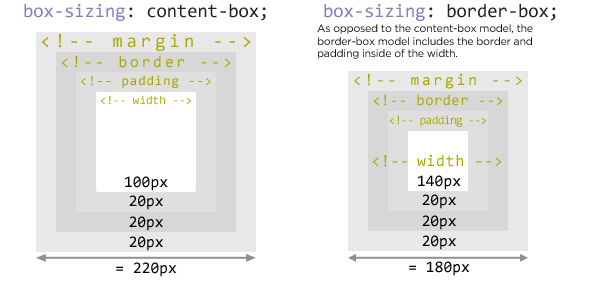
\includegraphics[scale=0.2]{box-model.png}

\css{vH}: \% der View-Height (\css{vW} Width, \css{20\%}: \% vom Parent, \css{calc(100vW - 5em)} berechnet.
\css{margin} kann auch negativ sein.

% Inline/Block/Inline-Block KURZ aufschlüsseln (05 20)
\subsection{Inline/Block/Inline-Block}
\textbf{Inline} wie \html{span a}, erlaubt left/right Margin/Padding, aber nicht top/bottom. Ignoriert width/height. Erlaubt andere Elemente auf der gleichen Zeile. White-Space zwischen Inline-Elementen wird dargestellt (Space). Forcieren: \css{display: inline}

\textbf{Block} wie \html{h1 div form p }, erlaubt Margin/Pading, jedes Element auf einer neuen ''Zeile'' (Umbruch), erlaubt Text-Inhalte zu scrollen, clippen (\css{overflow: scroll | hidden | invisible} Forcieren: \css{display: block}

\textbf{Inline Block} wie Inline-Flex, Inline-Table erlaubt Margin/Pading, erlaubt andere Elemente auf der gleichen Zeile mit Alignment (\css{vertical-align: top}), erlaubt width/height, White-Space zwischen Inline-Block-Elementen wird dargestellt (Space) Forcieren: \css{display: inline-block}

\subsection{Flexbox}
% Flex-Grundlagen: (05 28ff) (vorallem Detail Inline-Block und Kurzform)
\textbf{Container}:
\css{display: flex} / \css{display: flex-inline}. Alle Flex-Items verhalten sich wie \css{inline-block}.



% Flex Main Axis vs. Cross Axis Attribute (flex-grow usw, vs align-items) (05 35)

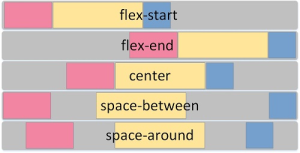
\includegraphics[scale=0.55]{flex-horizontal.png}
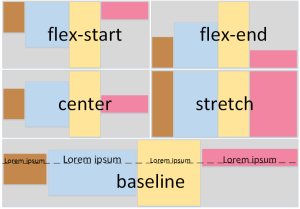
\includegraphics[scale=0.3]{flex-vertical.png}

\textbf{Main:} \css{justify-content} (Bild links)
\textbf{Cross:} \css{align-items} auf Container. Default: \css{flex-grow: stretch} (Bild rechts).

% Flex Wrap/Order/Direction (05 31-33)

Bei mehreren Zeilen \css{align-content:} mit allen properties wie \css{justify-content:}.

% Flex Begriff Main Axis/Cross Axis (05 34) LOW PRIO
\textbf{Ausrichtung:} Kann mit \css{flex-direction:} \css{row} (links-rechts) oder \css{column} (oben-unten) und mit \css{-reverse} auch die Reihenfolge geändert werden.

\textbf{Umbruch:} \css{flex-wrap:} \css{nowrap} (single line), \css{wrap} (wrap around additional lines), \css{wrap-reverse}. \css{flex-flow: [flex-direction] [flex-wrap]} kombiniert direction mit wrap.

% Flex-Eigenschaften (05 30)
\textbf{Grösse:} 
\css{flex-grow: 1}: entspricht dem Verhältnis, wie der ''leere Platz'' verteilt wird (default \css{0}, nicht grösser werden). \css{flex-shrink: 1}: entspricht dem Verhältnis, wie die Elemente kleiner werden, wenn zuwenig Platz (default \css{0}). \css{flex-basis: 100px | 10\% | auto}: gewünschte Start-Grösse des Elements (auch über \css{width/height} definierbar). Kurzschreibweise \css{flex: [flex-grow] [flex-shrink] [flex-basis]}

\textbf{Item:} Wenn ein Element in der falschen Reihenfolge ist: \css{order} default \css{0}. "Zuerst" werden die Elemente mit der kleinsten Order angezeigt. \textbf{Negative Elemente sind kleiner als 0 und nicht "vom Ende her" gezählt.} % TODO "Selektoren kennen nur die Source Order"
Dasselbe wie \css{align-items}  mit \css{align-self} auf dem einzelnen Item.

\subsection{Grid}
\textbf{Container:} 
\begin{minted}{css}
grid-template-columns: 1fr auto 20%;
grid-template-rows: repeat(4, 1fr);
\end{minted}

% Grid: Werte (05 50) KURZ
\textbf{fr}: Fraction of available Space, auch dezimal. Können nicht schmaler als das längste Wort werden. Overflow wird vermieden.

\textbf{max-content/min-content} grösst-/kleinstmöglich.

\textbf{auto} maximale gewünschte Breite der Grid-Elemente in der Spalte.

\textbf{minmax(min, max)}: Wert zwischen \css{min} und \css{max} wird sichergestellt. \css{minmax(auto, 1fr)}: soviel wie vom Inhalt vorgegeben wachsen mit \css{fr}.

\textbf{repeat(times: int, measure)} Wiederholung der \css{measure}, \css{grid-template-columns: 10em repeat(3, 1fr 2fr) 10em} => 8 Spalten: 10em, 3x (1fr/2fr) abwechselnd, 10em.

% Grid-Angaben (05 52) KURZ
\textbf{Item:}
\begin{minted}{css}
grid-column-start: 1; /* mit 1 indexiert */
grid-column-end: span 2; /* 2 ab -start */
grid-row-start: 2;
gird-row-end: -2; /* vis a vis gezählt */
grid-area: 2 / 1 / -2 / span 2; /* Kurzschreibweise */
/* [row-start]/[column-start]/[row-end]/[column-end] */
order: -2; /* default 0 */
\end{minted}

\textbf{template-areas}
\begin{minted}{css}
grid-template-areas: "aa bb bb" /* Container */
                     "aa . dd";
grid-area: aa /* Item */
\end{minted}

% Grid Element Alignment/Justification (Y/X) (05 54/55) KURZ
Element Alignment (Y): \css{align-items: stretch | start | center | end} (Default: \css{stretch}). Selber: \css{align-self}. Element Justification (X): \css{justify-items: stretch | start | center | end} (Default: \css{stretch}). Selber: \css{justify-self}.

% TODO Grid Holy Grail Layout (05 58) LOW PRIO TODO würde viel Platz brauchen...

\subsection{Media Queries}
% Media Queries Syntax (06 09-11)
\begin{minted}{css}
@media ([width|min-width|max-width]: 375px) {}
@media ([height|min-height|max-height]: 667px) {}
@media ([device-width|min-device-width|
    max-device-width]: 375px) {}
@media ([device-height|min-device-height|
    max-device-height]: 667px) {}
\end{minted}

\css{@media (orientation: landscape)}, oder \css{min-resolution: 300dpi}. Können auch kombiniert werden: \css{@media (min-width: 20em) and (max-width: 30em)} oder auch \css{@media only screen} (oder print).

% Standard Breakpoints (06 12) LOW PRIO
\textbf{Breakpoints:} \css{480px/30em}: Smartphones, \css{768px/48em}: Tablets, \css{992px/62em}: Desktops

% CSS Laden mit Media Queries (06 13) LOW PRIO
\textbf{Style Tag:} \html{<link rel="stylesheet" href="style.css" media="(min-width: 30em)">}

% Tipps/Tricks (06 18) LOW PRIO
Bei Texten \css{max-width: 60em} verwenden gegen überlange Zeilen. Media-Queries können in JS abgefragt werden: \js{if (window.matchMedia("(minWidth: 35em)").matches)}

\subsection{Viewport}
% Viewport setzen wenn Seite responsive ist, damit Media Query greift (06 20)
Bei einer responsiven Seite setzt man den Viewport, damit der Browser nicht "intelligent" versucht zu zoomen. Ohne, greifen die Media Queries nicht. \html{<meta name="viewport" content="width=device-width, initial-scale=1">}. \html{width=device-width}: die Seite soll so breit sein, wie das Gerät. \html{initial-scale: 1} zoome zu Beginn so, dass es 100\% entspricht.
% TODO ViewPort, was will er da konkret wissen? Aussage (06 21): "Details zu Viewport sind kein Lernstoff"

\section{Sass/SCSS}
% TODO: SASS to CSS, SASS & HTML zeichnen, Viewport (l: Viewport oben)
% TODO SASS vs. SCSS (07a 16) LOW PRIO
% SCSS Syntax (07a 18-30) jeweils KURZ Anweisung UND Beispiel
\verb|$| Variablen,
\verb|&| Parent-Selektor, 
\verb|%| Placeholder (Abstract), 
\verb|@| Steuerzeichen (\scss{@if}, \scss{@else}), 
\verb|#{}| Interpolation (p.\verb|#{$name}|),
\scss{/* */} und \scss{//} Kommentare.

\textbf{Variablen:}
\begin{minted}{scss}
$colorMain: #abcdef;
a { color: $colorMain }
\end{minted}

\textbf{Nesting:}
\begin{minted}{scss}
nav {
  ul { display: block }
  li { display: inline-block }
  > a { padding: 6px }
} /* => */
nav ul { display: block }
nav li { display: inline-block }
nav > a { padding: 6px }
\end{minted}

\textbf{Parent Selector}
\scss{&} wird durch Parent-Selektor ersetzt
\begin{minted}{scss}
.headline {
  margin-top: 5em
  .sidebar & { margin-top: 2em }
  &:hover { color: darkred}
} /* => */
.headline { margin-top: 5em }
.sidebar .headline { margin-top: 2em }
.headline:hover { color: darkred }
\end{minted}

\textbf{Partials/Imports}
müssen mit einem Underscore beginnen (\scss{_}), werden nicht in separates CSS übersetzt. Bei \scss{@import} muss die Dateiendung und der \scss{_} nicht angegeben werden.

\begin{minted}{scss}
// file: _constants
$brand-color: #abcdef
$width: 960px
// anderes File
@import 'constants'
h1 { color: $brand-color }
body { width: $width }
\end{minted}

\subsection{Mixins}
\scss{@mixin} definiert neues Mixin, \scss{@include} lädt das Mixin. Auch mit Parameter (und Default).
\begin{minted}{scss}
@mixin visuallyhidden($border: 1em) {
  border: $border
  height: 1px /* ... /*
}
.element {
  @include visuallyhidden(1rem)
}
\end{minted}
\scss{@content} wird mit dem Content von \scss{@include {}} abgefüllt. Auch mit Parametern nutzbar.
\begin{minted}{scss}
@mixin breakpoint($size) {
  @media screen and (min-width: $size) { @content }
}
@include breakpoint(30em) { ... }
\end{minted}
\scss{@content} wiederum kann beliebiges SCSS sein, inkl. Includes. Auch \scss{&} funktioniert richtig:
\begin{minted}{scss}
@mixin hover() { &:hover { background: red } }
.box { @include hover() } /* => */
.box:hover { background: red }
\end{minted}

\textbf{Extend/Inheritance}
\begin{minted}{scss}
.icon { margin: 0.5em }
.error-icon { @extend .icon; background: red }
.info-icon { @extend .icon; background: blue }
/* ==> */
.icon, .error-icon, .info-icon { margin: 0.5em }
.error-icon { background: red }
.info-icon { background: blue }
\end{minted}
Mit \verb|%| kann Abstract Class genutzt werden.  % l: kann man notfalls auch weglassen und textlich erklären
\begin{minted}{scss}
%icon { margin: 0.5em }
.error-icon { @extend %icon; background: red }
.info-icon { @extend %icon; background: blue }
/* ==> */
.error-icon, .info-icon { margin: 0.5em }
.error-icon { background: red }
.info-icon { background: blue }
\end{minted}

% TODO SCSS Mixins vs. Extends LOW PRIO (07a-31)
% SCSS Einheiten/rechnen (07a 33/34) LOW PRIO
\textbf{Einheiten / Rechnen}
Numbers (\scss{1, 1.2, 1px}), Strings mit oder ohne \scss{""}, Colors, Booleans, Nulls, Listen (mit Komma oder Leerzeichen, \scss{$list = 1.5em 1em 0 2em}), Maps: \scss{(k1: v1, k2: v2)}. Beispiele: \scss{2px + 2px = 4px}, \scss{2px/1px = 2}, \scss{2px + 1mm = 5.78px}, \scss{10 + px = "10px"} aber Achtung: \scss{10px * 10px = 100px*px = Error}

\textbf{Loops/Verzweigungen}
\begin{minted}{scss}
$width = 2px;
$breakpoints: 30em 46em
@each $point in $breakpoints {
  @media all and (max-width: $point) {
    body { 
      @if $point > 40 em { width: $width }
      @else { width: $width * 2 }
}}} /* => */
@media all and (max-width: 30em) { /* else */
  body { width: 4px }
}
@media all and (max-width: 46em) { /* if */
  body { width: 2px }
}
\end{minted}
\textbf{Funktionen}
\begin{minted}{scss}
@function properZero($param) {
  @if (komplizierte Rechnung mit $param) {
    return $param / komplizierte Rechnung
  } @else { return $param }
}
body { width: properZero(0px) }
\end{minted}

% CSS Variablen: Deklaration/Verwendung, Vererbung/Default erwähnen, übersteuern in Media Queries (LOW PRIO), abfragen in JS (LOW PRIO) (07b)
\subsection{CSS-Variablen (ohne SASS)}
Beginnen mit \css{--}. Da alle Properties sich dem DOM nach vererben, definiert man Custom Properties typischerweise auf dem Body, und nutzt sie dann später mit \css{var()}. Anders als Sass-Variablen, können sie zur Laufzeit abgefragt und geändert werden.
\begin{minted}{css}
body { --main-bg-color: red }
div { background-color: var(--main-bg-color) }
/* mit Default Wert */
div { background-color: var(--main-bg-color, red) }
/* auch mit calc */
body { font-size: calc(2 * var(--base-font-size)) }
/* übersteuern */
@media screen and (min-width: 560px) { 
  body { --main-bg-color: blue }
}
\end{minted}
% Variante: \js{getComputedStyle(element).getPropertyValue("--my-var")}
In JS abfragen: \js{element.style.getPropertyValue("--my-var")}, setzen: \js{element.style.setProperty("--my-var", jsVar + 4)}

\section{UCD}
% TODO: UCD Interaktionsmodell nach Norman, Methoden, Accessibility, Cognitive Walkthrough
% ACHTUNG Beim folgenden (08) kann ich mir nicht vorstellen, was er wirklich haben will. Habe darum nur aufgeschrieben, was allenfalls gut abfragbar ist. Wir müssen daraus noch rausfiltern, was wir wirklich drauf haben wollen...
% ACHTUNG Cognitive Walkthrough, ist nicht in der Vorlesung
% Accessibility ist nicht nur "mit Screenreader testen" (08 13-15)
Accessibility ist nicht nur "mit Screenreader testen"!

% Regeln (08 21-23)
\textbf{Regeln:} Jedem Bild und Animation Beschreibung zuordnen (\html{alt}), keine Informationen ausschliesslich mit Farbe darstellen, Vorder-/Hintergrund auch bei weniger Farbe/Konstrast deutlich unterscheidbar machen, Skalierung der Schrift (\html{em/rem/\%} statt \html{px}), Tastaturbedienung, Altersgerecht: leichter ablenkbar (keine Animation), Fonts unter 11pt kaum lesbar, Targets nicht zu klein, im DOM Navigation zuerst, Bereiche gruppieren, semantic Markup nutzen, komplementäre Farben vermeiden.

\textbf{Accessibility Tree} Der "Accessibility Tree" ist die von Screen-Readern genutzte, vereinfachte und mit Zusatzinformationen ausgestattete Repräsentation des HTMLs.


\subsection{Norman}
% Interaktionsmodell Norman (08 35)
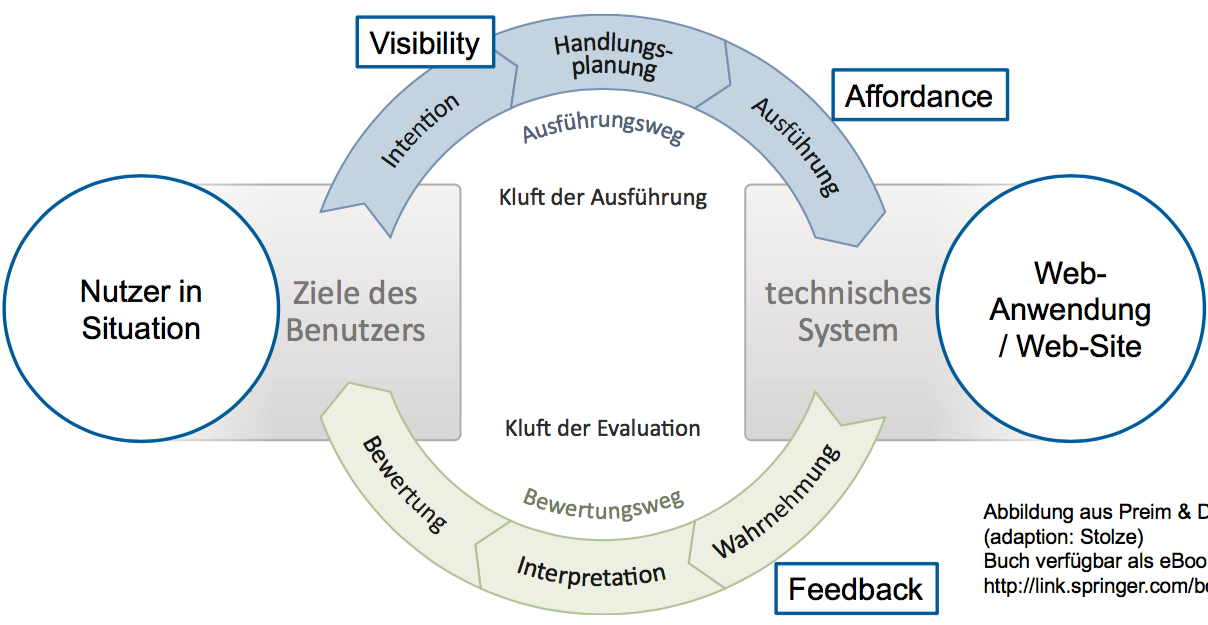
\includegraphics[scale=0.13]{norman.png}

% Kontrastverhältnisse (08 8)
\textbf{Kontrast} 15.9:1 für 80+, 5.7:1 für 50+.

% Begriff Affordance erklären (08 36ff, insb. 38)
\textbf{Affordance} wie kann ich etwas bedienen? Türen: Klinke, Hebel. Links blau unterstreichen. Logo oben links/rechts führt zur Homepage. Grauer Hintergrund-Text ist Label oder Instruktion. Login/Nutzerinformation ist oben rechts. Navigation-Menü ist oben. Such-Felder haben Lupe. Buttons sollen wie Buttons aussehen.
\textbf{Instruktionstexte sind Symptom für schlechte Affordance}.

% Card Sorting (08 47)
% Garrett Vorgehen/Wireframe (08 52/53)
\subsection{Card Sorting/Garrett/Wireframe}
\textbf{Card Sorting} (1) Content Repository erstellen, (2) \textbf{Open Card Sort:} 5+ Personen aus der Zielgruppe, Elemente in disjunkte Gruppen ordnen, (3) gute Gruppennamen identifizieren, (4) \textbf{Closed Card Sort:} validieren: 5+ neue Personen, Gruppennamen vorgeben, Elemente diesen Gruppen zuordnen lassen.
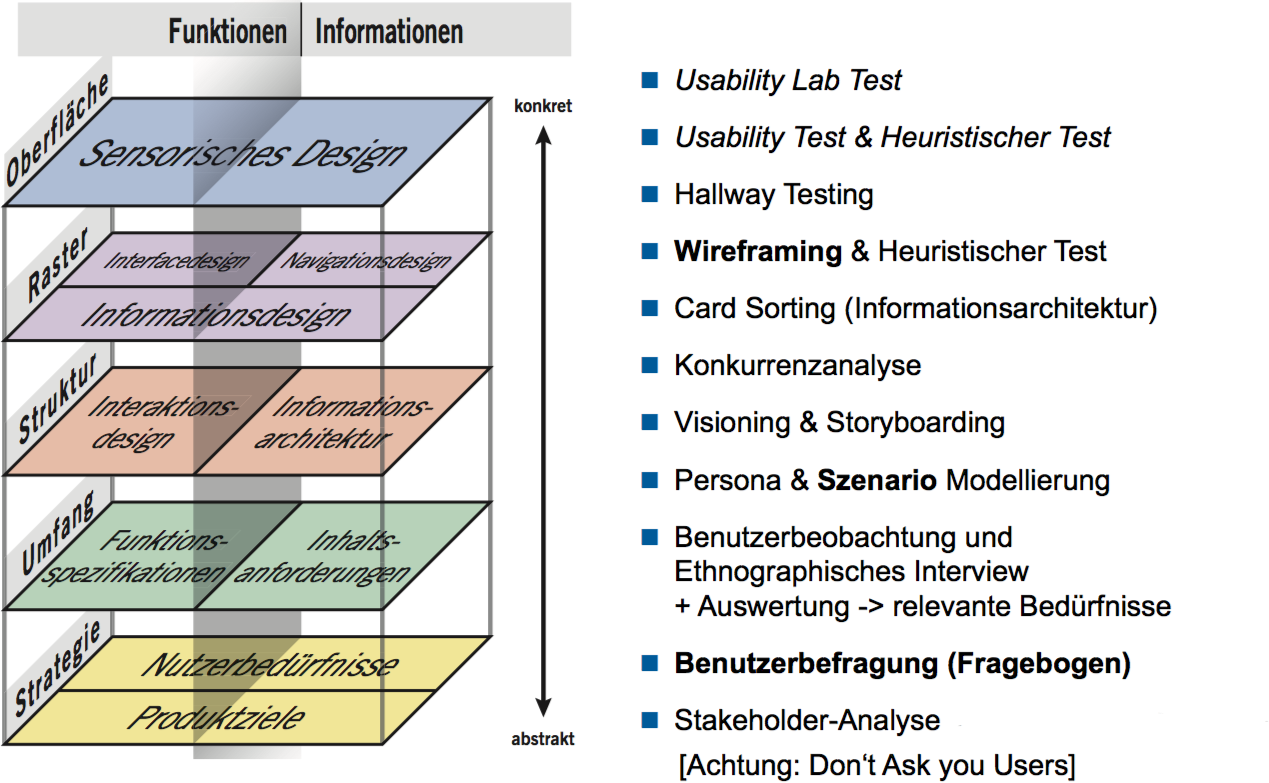
\includegraphics[scale=0.13]{Garrett.png}
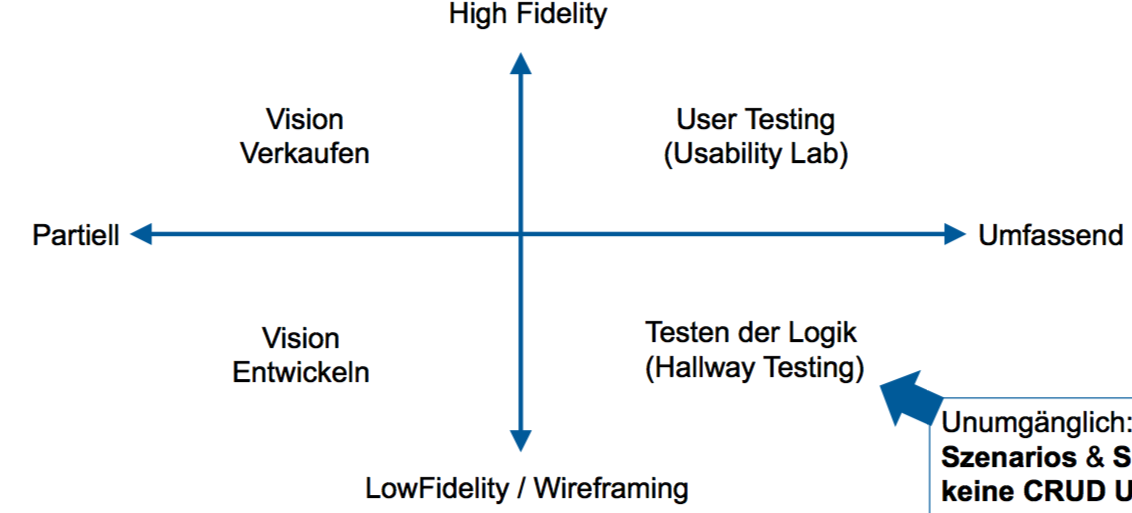
\includegraphics[scale=0.13]{Wireframing.png}

\subsection{Tree Testing} Zugeklappten Menü-Tree vorgeben, Nutzer Aufgabe geben "Finde X", sehen ob er es findet, und wo er sich durchhangelt.

\subsection{Kriterien}
Tastaturbedienbarkeit, semantische Struktur, Multimedia/2-Sinne Prinzip, Kontrast, Syntax/Kompatibilität, Hilfestellung bei Interaktionen

\section{Security}


% TODO: node.js Security Insecure Direct Object References, Cross-Site-Scripting, eval(), 
% TODO Repetitionsfragen in den Übungen W09 Abhandeln!
% ACHTUNG 09 kann man gut mit 1-2 Sätzen jeweils beschreiben. Für die konkreten Tipps besser TOST (= Top Overlooked Security Threats) verwenden
% XSS-Beschreibung (09 10) KURZ
\subsection{XSS Cross Site-Scripting}
In einem Formular angegebene Daten werden an andere Nutzer ohne Escaping ausgeliefert. 
% XSS mitigieren (TOST 20-27)
Encode for ... \textbf{HTML Body} \texttt{<} => \texttt{\&lt;}, \textbf{HTML Attributes} nicht-alphanumerisches: \text{\&\#xHH}-Format. \textbf{CSS} CSS Hex Encoding \texttt{\textbackslash HHHHH}, \textbf{JS} nicht-alphanumerisches \texttt{\textbackslash uXXXX}, \textbf{URI} \texttt{encodeURI}, \textbf{URL Parameter} \texttt{encodeURIComponent()}.
% XSS Lösung (09 11) LOW PRIO, (09 12) (normale PRIO)
% HTTPOnly, Content Security Policy (TOST 28/29
Ferner CSP setzen und httpOnly (nicht in JS auslesbar) + secure auf dem Cookie.

% JS Injection (09 17) Beispiel, Gegenmassnahme KURZ
\subsection{JS Injection}
Nie \js{eval} verwenden! Möchte man z.B. einen Zahlenstring in einem Request mit \js{eval} in eine Zahl verwandeln, so könnte ein Angreifer dort beliebiges JS platzieren und damit den Server übernehmen.

% Broken Authentication and Session Management (09 21-23) KURZ
\subsection{Broken Authentication and Session Management}
keine PW über HTTP, kurze Session Timeouts, keine ungehashten PWs

% Insecure Direct Object References Beispiel (09 26-27) KURZ
\subsection{Insecure Direct Object References}
Über eine manipulierte URL auf Daten zugreifen, für die man keine Berechtigung hat. Gegenmassnahme: sicherstellen, dass der Benutzer eingeloggt ist (Session-Token). 

\subsection{CSRF: Cross Site Request Forgery}
Bei einer Seite angemeldet sein, und eine fremde Seite sendet in meinem Namen Daten an die erste Seite.

\begin{minted}{js}
app.use(express.csrf())
app.use(function(req, res, next) {
 res.locals.csrftoken = req.csrftoken()
}
\end{minted}
\begin{minted}{html}
<input type="hidden" name="_csrf"
  value="{{csrftoken}}">}
\end{minted}

\subsection{Security by Obscurity}
Powered By ausschalten, Session Cookie Namen generisch machen.

\section{OO}
% JS kennt kein Overloading (10 06) LOW PRIO
JavaScript kennt kein Overloading! \textbf{Dieser Konstruktor (Factory-Methode) kann mit oder ohne \js{new} aufgerufen werden.}
\subsection{this}
\begin{minted}{js}
function newCounterWithInc(init) {
  const o = {}
  o.count = init
  o.inc = function(delta) { this.count += delta }
  return o
}
const c = newCounterWithInc(7)
c.inc(5)
\end{minted}


"Freie" Funktionen können mit \js{call/apply}, ferner \js{bind}, das \js{this} gesetzt bekommen.
\begin{minted}{js}
function globalCount(delta) { this.count += delta }
const o = {count: 1}
globalCount.call(o, 3)
\end{minted}
Unterschied \js{call/apply} bei \textbf{c}all gibt man die Argumente an die eigentliche Funktion mit \textbf{C}ommas weiter, bei \textbf{a}pply mit einem \textbf{A}rray.

Mit \js{bind} erhält man eine neue Funktion, deren \js{this} dauerhaft gebunden ist.
\begin{minted}{js}
const oFn = globalCount.bind(o)
oFn(3)
\end{minted}

% TODO Array-Problem (10 12) LOW PRIO
% TODO 10 15/16 verstehen
% TODO Objekteigenschaften (10 21) LOW PRIO

\subsection{ES5 Konstruktor}
% Konstruktoren (alt) (10 22)
Konstruktoren sind normale Funktion. Nach Konvention grossgeschrieben. Müssen mit \js{new} genutzt werden
\begin{minted}{js}
function Counter(cInit) {
  this.cont = cInit
  this.inc = function (delta) { this.count += delta }
}
const c = new Counter(12)
\end{minted}

% Prototypen (10 24/25) 
\subsection{Prototypes}
JS verwendet das System der Prototypen. Dabei gibt es eine Prototype Chain, entlang derer die gewünschte Methode/Property gesucht wird. Wenn sie gefunden wird, wird \js{this} auf das ursprüngliche Objekt gesetzt und die Methode aufgerufen. Man kann auch nachträglich bei einem früheren Prototyp eine Funktion anhängen; diese wird auch dann gefunden wenn sie bei der Konstruktion des neuen Objekts noch nicht bekannt war. Jedes mittels Konstruktor erstelltes Objekt hat einen Pointer auf das Prototyp-Objekt des Konstruktors (\js{.\_\_proto\_\_}

Mit den Prototypen kann eine mehrstufige Vererbung erzielt werden. Wird heute nicht mehr empfohlen, aber die ES2015 Syntax wird entsprechend übersetzt.

% können wir gerne auch wieder löschen
\begin{minted}{js}
function Shape() {}
Shape.prototype.getArea = function() {return 0;}
function Rect(width, length) {
  const r = {}
  r._width = width; r._length = length;
  r.getArea = function() {return r._width * r._length;};
  return r;
}
Rect.prototype = Object.create(Shape.prototype);
function Square(edgeLength) {
  const n = Number(edgeLength);
  // Nicht mit new aufgerufen
  if (this === window) { return new Square(n); }
  else { return new Rect(n, n); }
}
Square.prototype = Object.create(Rect.prototype);
\end{minted}

\textbf{Mit \js{new} oder ohne aufgerufen?} wenn \js{this === global} (im Browser \js{window}) ist, wurde es \textit{OHNE} new aufgerufen. 

% TODO Object Rest/Spread (10 31ff) KURZ/LOW PRIO
\subsection{ES6 Verbesserungen}
% Property getter/setter erwähnen (11 16)
% ES6 OO Klasse (11 19)
% ES6 OO Vererbung (11 21)
Richtige Klassensyntax und Properties mit Getter/Setter
\begin{minted}{js}
class Counter {
  constructor({start = 0, step = 1}) = {}) {
    this._count = start
    this._step = step
  }
  get count() { return this._count }
  set count(newCount) { myCount = newCount }
  inc(step = this._step) { this._count += step }
  dec(step = this._step) { this._count -= step }
}
class DoubleCounter extends Counter {
  constructor({start = 0, step = 1} = {}) {
    super({start, step})
    this._step = this._step * 2
  }
}
const dc = new DoubleCounter({step : 4})
dc.inc()
\end{minted}


\section{Funktionales JS/Array Funktionen}
% TODO: JS .sort(), .filter(), .reduce(), .map(), Object.keys(), Object.values(), .join(), .reverse(), .every()
% TODO Array Lücken vs. undefined (11 29) LOW PRIO
% Array Funktionen (11 32/33) LOW PRIO
\begin{minted}{js}
// Filter: a.Filter(fn(element, [index], [array])
  : boolean)
function getNumberArray(i) {
  return i.filter(e => typeof e === "number)
}
// Map: a.map(fn(element, [index], [array])
  : modifiedE)
function incrementAllNumbers(i, increment) {
    return i.map(e => e + increment)
}
// Reduce: a.reduce(
  fn(acc, element, [index], [array]): result, 
  startResult)
function sumAllNumbers(i) {
  return i.reduce((result, e) => (result + e), 0)
}
// Filter Duplicates
toRemove.reduce((acc, element) => acc.includes(element) 
  ? acc : acc.concat([element]), []).sort();

\end{minted}
\js{Object.keys(object)}: alle Attribut-Namen des Objekts, \js{Object.values(object)}: alle Attribut-Werte des Objekts, \js{Arrays.every(fn(e): boolean)}: prüfen, ob alle Elemente eines Arrays eine Funktion erfüllen.

\begin{minted}{js}
// Welche Personen praktizieren dieselben Hobbies
data.filter(e => e.indexOf(hobby) >= 0)
    .map(e => e.name);
data.reduce((result, item) => {
 const key = item.hobbies.sort().join(",")
 result[key]) ? result[key].push(item.name) 
              : result[key] = [item.name]
});
// Palindrom (maoam)
data === data.reverse()
// Filter Duplicates
data.filter((e, i, a) => a.indexOf(e) === i)
\end{minted}

\section{TypeScript}
\textbf{Achtung: Schreibt man eine Klasse, die von einer (in der Datei) später definierten Klasse erbt, gibt es einen Compiler-Fehler. Dasselbe mit Funktionen, da der Compiler sie zu diesem Zeitpunkt noch nicht kennt.}
% TODO: Typescript, TSFuckery, JS to TS, TS to JS
% TODO TS Vorteile (13 6/7) LOW PRIO

% TS Grundlagen (13 11), inkl. Detail any kann ALLEM zugewiesen werden
\subsection{Variablen}
Benötigen keine Typendeklaration, dann wird der Typ inferiert. Man kann sie explizit als \js{any} deklarieren, dann (1) können beliebige Variablen zugewiesen werden und (2) \textbf{Variable darf beliebigen anderen Variablen zugewiesen werden}. Um globale-Variablen aus nicht TS-Files zu nutzen, deklariert man sie mit \js{declare let SOMEGLOBALVAR}.
Ist ein Variablentyp einmal inferiert oder festgelegt, kann man andere Typen nicht mehr zuweisen:
\begin{minted}{ts}
let inferredNumVar = 1; inferredNumVar = "hi" // NOK
let numVar : number = 1; numVar = "hi" // NOK
\end{minted}
Möchte man eine Variable nur deklarieren, nutzt man \js{declare let foo: string}.

% TS Array, Tupels, Enums (13 12) KURZ
\subsection{Komplexe Typen}
Bei Arrays wird der Typ inferiert.
\begin{minted}{ts}
let infNumArray = [1, 2, 3]
let numArray: number[] = [1, 2, 3]
\end{minted}

Bei Tupeln ist dies nicht möglich
\begin{minted}{ts}
let notInfTupel = [1, 'abcd']
let tupel: [number, string] = [1, 'abcd']
\end{minted}

Enums können wie Basistypen genutzt werden
\begin{minted}{ts}
enum Color { Red, Green, Blue }
let c: Color = Color.Green
let colorTupel: [Color, number] = [Color.Green, 1]
\end{minted}

\subsection{Funktionen}
% TS Funktionen inkl. Overloading (13 13)
Hier auch mit Overloading! Und optionalen Parametern
\begin{minted}{ts}
function add(s1: string, s2: string): string
function add(n1: number, n2: number): number
function add(n1, n2) { return n1 + n2 }
function combineFunction(sn: number | string = "",
  ns?: number): string {
  return sn.toString() + (ns || "").toString()
}
\end{minted}
% TS Typ von Funktionen (13 14)
Auch Funktionen können als Parameter deklariert werden
\begin{minted}{ts}
function numberApplicator(numArray: number[],
  numFun: (prevResult: number, current: number)
  => number) :number {
  return numArray.reduce(numFun)
}
numberApplicator([1, 2, 3, 4], add)
\end{minted}
\subsection{Klassen}
% TS Klassen und Interfaces (13 15/16)
Erweiterte ES6 Syntax inkl. Properties und \js{private}/\js{readonly}. \js{private} kann überschrieben werden.
\begin{minted}{ts}
class Counter {
  private _doors: number
  public static readonly WOOD_FACTORS = 
    { 'oak': 80, 'pine': 20}
  constructor({doors = 2}: {doors?: number} = {}) {
    this.doors = doors;
  }
  set doors(newDoorCount: number) {
    if(...) { this._doors = newDoorCount }
    else { throw '...' }
  }
  get doors() { return this._doors) }
}
\end{minted}
Vererbung und Interfaces. Klassen können in der Konstruktor-Argumentliste angeben, ob ein Parameter ein public/private Property sein soll. Dann spart man den Initialisierungscode.
\begin{minted}{ts}
interface IPoint { 
  readonly x: number; readonly y: number
}
interface ILikableItem { likes? : number }
class DescribableItem {
  constructor(public description: string) {}
}
class POI extends DescribableItem
  implements IPoint, ILikableItem {
  constructor(public x: number, public y: number,
    description: string, public likes?: number { 
    super(description)
  }
}

\end{minted}
% TODO TS Module (13 17), oder auch: "deckt sich mit ES6 Modul Syntax"
% TODO TS Custom Type (13 19)

% TS null/undefined (13 20)
\texttt{--strict} enables \texttt{noImplicitAny}, \texttt{noImplicitThis}, \texttt{strictNullChecks} (\js{null} and \js{undefined} values are not in the domain of every type and are only assignable to themselves) and \texttt{strictFunctionTypes} (contravariantly instead of bivariantly).

\begin{minted}{ts}
let a: any = true
let nb: number | boolean = "aaa" // fails
const nai = [3, 7, 9]
nai[6] = true // fails
let t: [number, boolean] = [42, false]
enum Decision { yes, no }
let y: Decision = Decision.no
declare let m: number
m = true // fails
function f(n1: number, n2?: number) {} // n2 optional
f(2) // ok
f(2, "ab") // fails
f(2, 3, 7) // fails
\end{minted}

\texttt{tsc --target 'ES6' f.ts} erstellt ein ES6 JS anstatt ein ES3.

\section{Testing}

% TODO: Testing TDD, TDD Circle, Jasmine
% ACHTUNG TDD Circle in Vorlesungen nicht erwähnt, Jasmine in Vorlesungen nicht erwähnt (Mocca und Expect)
% Unit Testing Phasen (14 13)
\subsection{Phasen}
Ein Unit Test hat vier Phasen: (1) Setup, (2) Exercise, (3) Verify, (4) Teardown
% Grundlagen Mocha und Beispiel-Test (14 16)
\subsection{Mocha}
Test-Beschreibungen geschachtelt.
\begin{minted}{js}
describe('Array', function() {
describe('#indexOf()', function() {
  beforeEach(function() { this.testArray = [1, 2, 3]});
  it('should return ...', function() {
    expect(this.testArray.indexOf(4)).toBe(-1))
  }); // weitere it()...
}); // weitere describe()...
});
\end{minted}

% expect.js API (KURZ) (14 18)
\subsection{Expect API}
\js{expect(x). toBe(val). toEqual(val). toThrow(err). toExist(). toBeTruthy(). toNotExist(). toBeFalsy()}

\subsection{Spies API}
\begin{minted}{js}
const video = { play: () => {...} }
spy = expect.spyOn(video, 'play')
expect(spy.calls.length).toEqual(1)
expect(spy.calls[0].context).toBe(video)
\end{minted}
\js{spy.expectSpyOn(...). andCallThrough(). andCall(fn). andThrow(exception) .andReturn(value)}

Stub-Werte zurückgeben: \js{spyOn(Date, 'now').andReturn(currentDate)} (\js{currentDate} fixiert).

% TODO TDD Prinzipien (KURZ) 14 20/21)
% Bei den folgenden Test-Pattern könnte man jeweils in einem Satz erklären und ein kleines Beispiel machen. Aber alles sehr kurz

\subsection{Test Pattern}
% Test Double Pattern inkl. DOC (depended-on Component) (14 22/23)
% Test Stub Pattern inkl. Spy-Einführung (14 24/25)
% Test Spy Pattern (14 26/27)
% Test Fake Object Pattern (14 28/29)
% Test Mock Object
\textbf{Test Double Pattern} DOC (depended-on Component) mit einem Interface ersetzen und einmal real und einmal als Double implementieren.


\textbf{Test Stub Pattern}
Immer dasselbe zurückgeben.

\textbf{Test Spy Pattern}
\begin{minted}{js}
class BankAccount { withdraw() {}, deposit() {} }
describe('A new transaction executed', function() {
  beforeEach(function() {
    this.accountA = new BankAccount()
    this.accountB = new BankAccount()
    spyOn(this.AccountA, 'withdraw')
    this.transaction =  new Transaction(
      this.accountA, this.accountB, 25)
  });
  it('withdraws 25 from account A', function() {
    this.transaction.execute()
    expect(this.accountA.withdraw).
      toHaveBeenCalledWith(25)
  });
});
\end{minted}

\textbf{Fake Object Pattern}
Z.B. einen Fake Hash Service bauen, der immer auf dem gleichen Seed operiert. Unterschied zum Stub ist sehr fein.

\textbf{Mock Object Pattern}
Objekt, das sich selber verifizieren kann, das wir dann fragen können ob alles korrekt lief

\subsection{Empfehlungen}
\textbf{Pure Functions}: Testbarkeit optimal, wo nötig Test Doubles als Argumente übergeben. \textbf{Non-pure Functions/JS Objekte}: Context für Test fixieren, globale Variablen setzen, Veränderung globaler Variablen überprüfen, Veränderung der Input-Argumente überprüfen, wo nötig Test Doubles als Argumente übergeben.

% TODO Unit Code Smells (14 34-40) KURZ l: wollen wir die?

\section{NodeJS/Express Fakten}
% Module Import (02 27) Suchreihenfolge
% node_modules nicht ausliefern (02 28) -> d: evtl.ein kurzer satz
\textbf{Module}
\textbf{Suchreihenfolge} 1. Core-Module, 2. falls mit Slash/Punkt am Anfang: (a. File, b. Directory), 3. falls Filename (\texttt{require('mymodule')}): in node\_modules, danach bis zum System Root.    
\textbf{node\_modules} nicht ausliefern! Kann Binary-Teile beinhalten, besser in package.json.

% (03 14), erwähnen dass Reihenfolge die Ausführungsreihenfolge bestimmt
\textbf{Middleware}
Die Reihenfolge der Registrierung bestimmt die Ausführungsreihenfolge.
% (03 20) erwähnen dass mehrere möglich sind
\textbf{Static Middleware} es sind auch mehrere static-Routes möglich.
% Error Middleware (03 22)
\textbf{Error-Middleware} muss als letztes registriert werden. Es können mehrere sein, die letzte muss die Anfrage beenden. Wird aufgerufen, wenn Error-Objekt dem Callback übergeben wird. Signatur wie normale Middleware, aber zusätzlicher erster Parameter \texttt{error}

% d: Ordnerstruktur (03 24)
\textbf{Ordnerstruktur vs. Architektur}

\texttt{/routes} \textbf{Entry point} Front Controller (does routing).
\texttt{/controller} \textbf{Controller}.
\texttt{/services} \textbf{Model}.

% Token als Session/Authorisierung erwähnen (03 41), JWT erwähnen (03 43/44) LOW PRIO
\textbf{Token} Idee: bei jeder Anfrage ein Token mitgeben. Bildet Berechtigungen ab, hat Ablaufdatum. Bsp: JSON Web Token (JWT).

\subsection{ES6 Module}
% Vorteile/Beschreibung von Module (12 05) LOW PRIO
Besitzen eigenen Scope. Ermöglicht Kapselung und lazy-loading. 
% Konventionen Module (12 08) LOW PRIO
Konventionen: 1 File = 1 Modul (= 1 Unit für Tests); 1 Folder = 1 Package = Sammlung von zusammengehrenden Modulen und Klassen.
% TODO Tier-Architektur Web (12 09) (gut abfragbar) LOW PRIO
% Module importieren und exportieren (12 11), deckt sich evtl. teilweise mit Anfang NodeJS
% TODO weitere Beispiele für Import/Export, (03 14) wäre komplette Syntax, aber das ist mir zu lang...
% ES6 Eigenschaften von Modulen (12 16)
% ES6 Module in Node verwenden (12 20/21) LOW PRIO
Modul-Import/Export Syntax ist leicht anders als NodeJS/CommonJS. Module sollten Endung \texttt{.mjs} haben. Sie werden im Strict-Mode interpretiert. Nur einmal geladen. Können nur mit Flag \texttt{--experimental-modules} in Node genutzt werden, Node unterstützt keine Dynamic Imports.
% ES6 Module Beispiel (12 17)
\begin{minted}{js}
// lib.mjs
export function add(x, y) { return x + y}
// main.js
import {add} from './lib.mjs'; add(2, 3)
\end{minted}

% Dynamic Imports (12 22)
\textbf{Dynamic Import} \texttt{'./main1.mjs'} definiert \texttt{global.DEMO\_VAR = 'MAIN1'}.
\begin{minted}{js}
import('./main1.mjs').then(() => {
  console.log(global.DEMO_VAR);
});
\end{minted}

\textbf{ES6 Module im Browser} können mit \html{<script [src=''] type='module'>[source]</script>} geladen werden.

% TODO Scoping in CommonJS Modulen (12 12)
% TODO (12 18/19) verstehen und evtl. einbinden
% TODO Revealing Module Pattern (12 27/28)
% ES6 Module im Browser laden (inkl. type=module) (12 33-35)

\subsection{Streams}
\begin{minted}{js}
let server = http.createServer(function (req, res) {
  let stream = fs.createReadStream(__dirname + '/d.txt');
  stream.pipe(res);
});
\end{minted}

\subsection{Events}
\begin{minted}{js}
const EventEmitter = require('events').EventEmitter;
class Door extends EventEmitter {
  constructor(){ super(); } 
  ring() { setTimeout(() => { this.emit('open'); }, 
    100); };
}
\end{minted}

\subsection{SOP/CORS}
Die \textbf{S}ame \textbf{O}rigin \textbf{P}olicy erlaubt XHR-Requests nur zur Origin. Mit \textbf{C}ross-\textbf{O}rigin \textbf{R}esource \textbf{S}haring kann man Cross-Site Requests ermöglichen. Chrome erlaubt kein CORS nach Localhost.

% CODE node Streams (02 33/34) LOW PRIO
% CODE node Events (02 35)

\section{NodeJS/Express}
\begin{minted}{js}
// app.js
var express = require('express')
var bodyParser = require('body-parser')
var session = require('express-session')
var app = express()
app.set('views', path.join(__dirname, 'views'))
app.set('view engine', 'hbs')
app.use(bodyparser.urlencoded())
app.use(cookieParser())
app.use(session({secret: 'abc', resave: false,
  cookie {secure: true}})
app.use(express.static(path.join(__dirname, 'public')))
app.use('/', require('./routes/search'))
app.use((req, res, next) => { // catch 404
  const err = new Error('Not found'), err.status = 404;
  next(err) // will skip to error middleware
});
app.use((err, req, res, next) => {
  res.status(err.status | 500)
  res.render('error')
});
module.exports = app
// routes/search.js
const express = require("express")
const router = express.Router()
const controller = 
  require("../controllers/searchController")
router.get("/", (req, res, next) =>
  controller.index(req, res))
// ODER router.get("/", controller.index)
router.get("/*", (req, res, next) =>
  controller.index(req, res))
router.get("/search", (req, res, next) =>
  controller.search(req, res))
module.exports = router
// public/js/autocomplete.js
$(() => {
  $("#searchText").keyup(() => {
    const searchText = $("#searchText").val()
    const searchType = $("#searchType").val()
    const resultContainer = $("#resultContainer")

    $.getJSON(
`/search?searchText=${searchText}&searchType=${searchType}`,
      data => {
        if (searchType === "person") {
          // person
        } else {
          resultContainer.empty()
          data.result.forEach(element =>
            resultContainer.append(
              new Option(element.title))
)}})})})
//controllers/searchController.js
const service = require("../services/searchService")
index = (req, res) => {
  res.render("index", { title: "Suche", 
    hasResult: false })
}
const isPersonSearch = typeString => 
  (typeString === "person" ? true : false)
const getTitleString = isPersonSearch =>
  isPersonSearch ? "Personensuche" : "Textsuche"
search = (req, res) => {
  const searchText = req.query["searchText"] || ""
  const searchType =
    isPersonSearch(req.query["searchType"])
  const searchResult = 
    service.search(searchText, searchType)
  res.format({
    "text/html": () =>
      res.render("index", {
        title: getTitleString(searchType),
        hasResult: true,
        isPersonSearch: searchType,
        searchResult: searchResult
      }),
    "application/json": () => 
      res.send(JSON.stringify(searchResult)),
    default: () => res.status(406).send("Not Acceptable")
  })
}
module.exports = { index, search }
\end{minted}
\begin{minted}{html}
// index.hbs
<script src='js/autocomplete.js'></script>
<form action="/search" method="get">
  <label>
  Suche<input name="searchText" id="searchText" 
    list="resultContainer"></label>
  <select name="searchType" id="searchType">
    <option value="text">Text Suche</option>
    <option value="person">Personen Suche</option>
  </select>
  <button>Suchen</button>
</form>
<datalist id="resultContainer" />
<h1>{{title}}</h1>
{{#if isPersonSearch}}
<table class="table">
  <thead>
    <tr><th><!-- Name, Email, Institut --></th></tr>
  </thead>
  <tbody>
    {{#each searchResult.result}}
    <tr>
      <td>{{this.name}}</td>
      <td><a href="mailto:{{this.email}}">
      {{this.email}}</a></td>
      <td>{{this.institut}}</td>
    </tr>
    {{/each}}
    </tbody>
</table>
{{else}} {{#each searchResult.result}}
<h4>{{this.title}}</h4>
<a href="{{this.link}}">{{this.link}}</a>
<p>{{{this.text}}}</p>
{{/each}} {{/if}}
\end{minted}

% TODO: Express App (autocomplete, controller, session,

% LOW PRIO FAKTEN
% Request/Response-Methoden (02 23/24) LOW PRIO
% Express: was wird Request/Response hinzugefügt (03 16) LOW PRIO
% AJAX XHR, fetch, jQuery.Ajax (03 49-51) LOW PRIO
% SOP/CORS (03 52/53) (in der Vorlesung als Einschub, nicht sicher wie wichtig in der Prüfung).
% Websockets (03 55) (wird in Vorlesung nicht beschrieben)

% BEISPIELE IM CODE
% DONE CODE Module Export (02 26) 
% CODE Module Import (02 27)
% DONE Express Start-Beispiel (03 12) -> d: evtl. überflüssig falls wir sowieso ein beispiel haben
% DONE CODE Middleware registrieren (03 14)
% DONE CODE Express Router: erstellen (2 Zeilen) und Methoden (03 18/19)
% DONE CODE Static Middleware Beispiel: "app.use(express.static(__dirname + '/public'))" (03 20)
% DONE CODE Custom Middleware schreiben (03 21)
% DONE CODE Datenhaltung: nedb, erstellen und Methoden (03 26/27)
% DONE CODE Express kann rendern, Render-Engine setzen (03 31)
% CODE Cookie/Session Methoden (03 34) LOW PRIO
% DONE CODE Unterschiedliche Formate im Router (03 40)
% Grösseres TODO: aus Demos von Vorlesung 3 Sachen herauspicken: https://github.com/gfeller/Vorlesung_Express

\paragraph{Value mit Priorität setzen} Hier: 1. Query, 2. Session, 3. Default 
\begin{minted}{js}
const getValueFromQuerySessionDefault = 
(query, session, defaultValue) =>
  query !== undefined ? query
  : session !== undefined ? session
  : defaultValue
// Anwendung
req.session.bla = getValueFromQuerySessionDefault(
  req.query.bla, req.session.bla, "Default Wert")
\end{minted}

\paragraph{Datalist für Autovervollständigung}
\begin{minted}{html}
<label>Choose a browser from this list:
<input list="browsers" name="myBrowser" /></label>
<datalist id="browsers">
  <option value="Chrome">
  <option value="Firefox">
  <option value="Internet Explorer">
</datalist>
\end{minted}

\paragraph{Number-Input}
\begin{minted}{html}
<input type="number" step="1" min="1" max="99" />
\end{minted}

\section{NeDB}
NeDB gibt jedem Doc eine ID unter \texttt{\_id}. Errors abfangen: \js{err ? console.log(err.message) : cb(...))}
\begin{minted}{js}
const Datastore = require('nedb')
const db = new Datastore({filename: './d.db',
  autoload: true}) // no need to load
const add = (note, cb) => {
  db.insert(note, (err, newDoc) => cb(newDoc))
}
const getNote = (id, cb) => {
  db.findOne({_id: id}, (err, newDoc) => cb(newDoc))
}
const getAllByDueDateThenImportance = cb => {
  return db.find({finished: true}) // {} for all
  .sort({dueDate: 1, importance: -1})// -1 reversed
  .exec((err, docs) => cb(docs))
}
const updateNote = (id, newNote, cb) => {
  db.update({_id: id}, newNote, 
    {returnUpdatedDocs: true},
    (err, count, doc) => cb(doc))
}
const removeNote = (id, cb) => {
  db.remove({_id: id}), // can be any query
  {multi: true}, // delete multiple matching
  (err, count) => cb()
}
\end{minted}


\end{multicols*}
\end{document}
